\section{Análisis de cluster}

\noindent Según Jain y Dubes  el análisis de \emph{cluster} es un conjunto de técnicas exploratorias que toman un conjunto de datos resultantes de recoger $N$ observaciones sobre $p$ medidas diferentes y buscan agrupar las observaciones. También se puede utilizar agrupaciones de variables pero no se desarrollará.

\noindent Para empezar, debemos definir que es un \emph{cluster}. Como en nuestro caso no buscamos agrupar variables, sino observaciones o mediciones utilizaremos la definición dada en \cite{Everitt 2011}.

\begin{defi}
Diremos que un \emph{cluster} o conglomerado es un subconjunto de las observaciones que son similares entre sí. 
\end{defi}

\noindent Es fácil observar que los clusters definen la siguiente relación de equivalencia $\mathcal{R}$ en la que dos observaciones, $\mathbf{x}_i,\mathbf{x}_{i'}, i,i'=1, \ldots, N$ están relacionadas si pertenecen al mismo clúster \cite{Cuadras 2014}. Por tanto, cada \emph{cluster} genera una clase de equivalencia $[c_k], k=1\ldots K$ donde $K$ es el número de clusters

\noindent El conjunto de \emph{clusters} generan un \emph{clustering} o partición , es decir:
\begin{defi}
Se llama \textit{clustering} a la partición que provoca la relación $\mathcal{R}$ del espacio de observaciones. 
\end{defi}

\noindent Para llegar a dichas particiones podemos usar distintos tipos de algoritmos según el número de particiones distintas que se generen a lo largo del proceso \cite{Jain 1988}:
\begin{itemize}
\item Particional Son aquellos procesos de \emph{clustering} en los que de manera previa se conocen el número de \emph{clusters} y por tanto, se genera una partición que se va modificando.
\item Jerárquico, si el proceso genera una secuencia anidada de particiones, es decir, que dependiendo de cómo se desarrolle puede ser de los siguientes tipos:
\begin{itemize}
\item Aglomerativo Cuando se inicia con una partición que tiene $N$ \emph{clusters} con una observación en cada uno. Este tipo de algoritmos va tomando los \emph{clusters} y junta aquellos según un criterio establecido hasta llegar a un criterio de parada. 
\item Divisivo Cuando empieza con un único \emph{cluster} que contiene a las $N$ observaciones. En cada paso se va dividiendo los cluster siguiendo algún criterio hasta llegar al criterio de parada. 
\end{itemize}
\end{itemize}

\noindent En resumen, el análisis de cluster es un conjunto de técnicas que permiten la simplificación estructural de las observaciones recogidas de un vector aleatorio mediante la agrupación de las mismas en conjuntos llamados clusters \cite{Everitt 2011}. 

\noindent El análisis de clusters ha sido aplicado en infinidad de áreas como el marketing con el objetivo de segmentar los anuncios \cite{Okazaki 2006}, la psicología para detectar si se da un sólo trastorno en una población \cite{Everitt 2002} o en el caso de la medicina para intentar estudiar la supervivencia de pacientes con carcinoma renal \cite{Witten 2010}. Estos son ejemplos de unas pocas aplicaciones, pero también nos pueden ayudar en la predicción del riesgo crediticio, segmentación electoral etc... 

\subsection{Algoritmos jerárquicos}

\noindent Los algoritmos jerárquicos calculan en cada paso la similaridad o disimilaridad entre \emph{clusters} para generar nuevas particiones del espacio uniendo o separando los distintos \emph{clusters}.

\noindent Un algoritmo jerárquico genera una secuencia de particiones anidada que está definida de la siguiente manera \cite{Scitovski 2021} :
\begin{defi}
Una partición del espacio $\Pi^{(r)}$ está anidada en otra partición $\Pi^{(k)}$ y se denota $\Pi^{(r)} \sqsubset \Pi^{(k)}$ si cumple lo siguiente:
\begin{itemize}
\item El número de clusters de $\Pi^{(k)}$ es menor que el de $\Pi^{(r)}$. 
\item Cada cluster de la partición $\Pi^{(r)}$ es un subconjunto de algún cluster de $\Pi^{(k)}$. 
\end{itemize}
En el caso de un algoritmo aglomerativo tendremos que $k>r$, es decir en el paso $k$-ésimo el número de \emph{clusters}.

\end{defi}

\noindent La pregunta que hay que hacer antes de aplicar este tipo de algoritmos, es cómo calcular las distancias o similaridad entre dos observaciones. Hay que distinguir dos casos, el cálculo inicial de las distancias entre observaciones del espacio y la distancia entre \emph{clusters}. Dependiendo de como se elijan sobre todo las últimas se tendrá un algoritmo de \emph{clustering} u otro \cite{Peña 2002}. 

\noindent En particular los métodos jerárquicos se pueden aplicar a distancias y similaridades, (veáse \cite{Mardia 1979}) Estas se pueden definir de distintas formas pero la más habitual es la distancia de Mahalanobis como se detallaba en la definición \ref{Mahalanobis}. Aunque esta sólo se detalla para variables continuas. 

\noindent Dependiendo de como se defina dicha distancia va a provocar que tengamos uno u otro tipo de algoritmo jerárquico.\cite{Everitt 2011, Johnson 2007, Peña 2002}
\begin{itemize}
\item El vecino más proximo: $d(C,C')=\min_{\mathbf{x}_i\in C, \mathbf{x}_{i'}\in C'}(\mathbf{x}_i,\mathbf{x}_{i'})$, es decir, se toma como la distancia entre los \emph{clusters} y una observación, $\mathbf{x}_{i'}$, el mínimo de las distancias entre las observaciones del propio cluster y la observación considerada.
\item El vecino más lejano: $d(C,C')=\max_{\mathbf{x}_i\in C, \mathbf{x}_{i'}\in C'}(\mathbf{x}_i,\mathbf{x}_{i'})$, es decir, se toma como la distancia máxima entre todas las posibles. 
\item Enlace medio \begin{equation}
d(C,C')=\dfrac{1}{N_C}\dfrac{1}{N_C'}\sum_{\mathbf{x}_i\in C}\sum_{\mathbf{x}_{i'}\in C'} d(\mathbf{x}_i, \mathbf{x}_{i'})
\end{equation}
donde $N_C, N_{C'}$ son el número de observaciones que hay en cada cluster. Es decir, es la media de todas las distancias. 
\item Ward:
\begin{equation}
d(C,C')=\dfrac{1}{N_C}\dfrac{1}{N_C'}\sum_{\mathbf{x}_i\in C}\sum_{\mathbf{x}_{i'}\in C'} (d(\mathbf{x}_i, \mathbf{x}_{i'}))^2
\end{equation} 

donde $N_C, N_{C'}$ son igual que antes. En particular, el algoritmo de Ward calcula las variación en los \emph{clusters}
\end{itemize}

\noindent En general, un algoritmo jerárquico aglomerativo funciona de la siguiente manera:

\begin{itemize}
\item Se inicia con una partición que tiene $N$ \emph{clusters} con una única observación cada uno.
\item Se calcula la matriz de distancias entre los \emph{clusters}. 
\item Se unen los dos clusters que menor distancia tengan entre ellos. De esta manera, se reduce el número de clusters en 1.  
\item Se repiten los dos pasos anteriores hasta tener u
n único cluster. 
\end{itemize}

\noindent El resultado de estos algoritmos es un dendograma \cite{Mardia 1979}
\begin{defi}
Un dendograma es un diagrama de árbol en el que en el eje horizontal se situan las observaciones mientras que en el eje vertical se representan las distancias. Cada nodo representa una unión de los clusters. 
\end{defi}

\noindent Los siguientes dendogramas \ref{fig:complete_linkage} \ref{fig:single_linkage}  son resultado de aplicar un algoritmo jerárquico al conjunto \emph{IRIS} de Fisher \cite{Iris Fisher}.
\begin{figure}[h]
 \centering
  \subfloat[Enlace completo]{
   \label{fig:complete_linkage}
    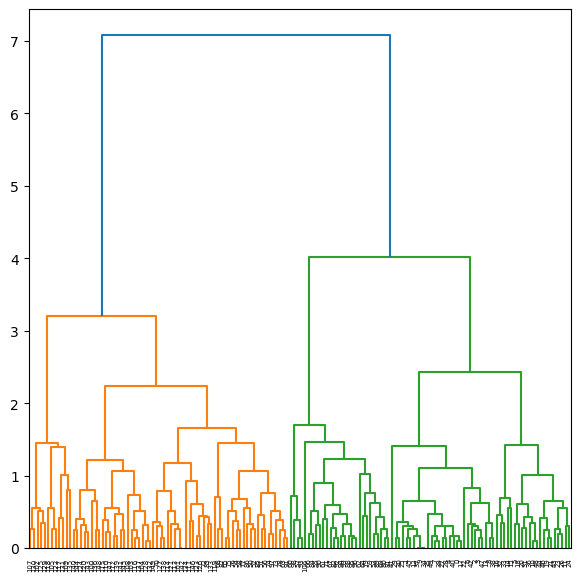
\includegraphics[width=0.3\textwidth]{Documentos Extra/Imagenes/complete_linkage.png}}
  \subfloat[Enlace simple]{
   \label{fig:single_linkage}
    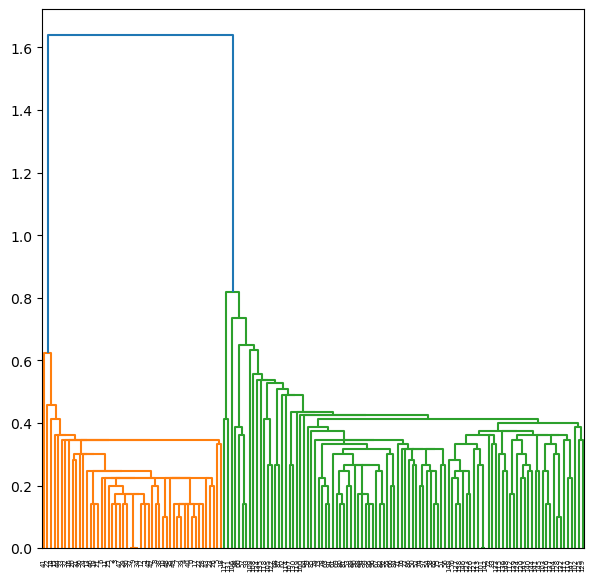
\includegraphics[width=0.3\textwidth]{Documentos Extra/Imagenes/single_linkage.png}}
 \caption{Diagramas obtenidos utilizando la biblioteca de Python Scikit-Learn}
 \label{fig:Dendogramas distintos enlaces }
\end{figure}
\subsection{Algoritmos particionales}

\noindent Dada una matriz de datos $\mathbf{X}$ de tamaño $N\times p$ resultado de realizar $N$ observaciones de $p$ variables aleatorias. El \emph{clustering} particional busca hacer una partición que divida las observaciones en $K$ grupos homogéneos 

\begin{defi}
Se llama \emph{centroide} de un cluster $C_k,\quad k=1,\ldots,K$ al vector de tamaño $p$ cuyas componentes son las medias de cada una de las variables de todas las observaciones del \emph{cluster} $C_k$:
\begin{equation}
\overline{x}_{jk}=\dfrac{1}{|C_k|}\sum_{i\in C_k}  x_{ij} \quad \forall j=1,\ldots, p
\end{equation}
\end{defi}

\noindent El algoritmo de $K$-medias es el más importante de este tipo \cite{Johnson 2007}. Se desarrolla de la siguiente manera  :
\begin{enumerate}
\item Se asigna a cada una de las observaciones en cada uno de los $C$ \emph{clusters}. Se calculan los centroides de dichos \emph{clusters}.
\item Se comprueba la distancia euclidiana de cada una de las observaciones a los centroides de los \emph{clusters} y se reasignan las observaciones de acuerdo al \emph{cluster} más cercano. Tras esto se recalculan los centroides.
\item Se repiten los dos pasos anteriores hasta que las asignaciones no cambien. 
\end{enumerate}

\noindent Resaltar que este algoritmo tiene un problema y es que los resultados finales 

\noindent Hay otras alternativas que utilizan criterios de variabilidad intra grupos o entre grupos para realizar las asignaciones óptimas fijados el número de clusters, para ello léase \cite{Everitt 2011, Peña 2002, Hartigan 1975}







